\documentclass{bioinfo}
\copyrightyear{2023} \pubyear{2023}



% tightlist command for lists without linebreak
\providecommand{\tightlist}{%
  \setlength{\itemsep}{0pt}\setlength{\parskip}{0pt}}




% hyperref makes the margins screwy.
% https://groups.google.com/forum/#!topic/latexusersgroup/4W_SwGk6zx4
% http://ansuz.sooke.bc.ca/software/latex-tricks.php
% \usepackage[colorlinks=true, allcolors=blue]{hyperref}

\access{Advance Access Publication Date:   }
\appnotes{Application Note}

\begin{document}


\firstpage{1}

\subtitle{Multi-Omic analysis}

\title[Multi-Omic Bioinformatics]{Elucidating Amphotericin B resistance
in \emph{L. }mexicana promastigotes using a Multi-Omics approach}

\author[FirstAuthorLastName \textit{et~al}.]{
2117832\,\textsuperscript{1}
}

\address{
\textsuperscript{1}University of Glasgow, Glasgow, G12 8QQ, Scotland\\
}

\corresp{}

\history{Received on XXX; revised on XXX; accepted on XXX}

\editor{Associate Editor: XXX}

\abstract{
\textbf{Motivation:} Leishmaniasis is a neglected tropical disease that
affects millions of people across the globe. A repurposed anti-fungal
drug, Amphotericin B, is being increasingly used to treat for
Leishmaniasis. Recently, there have been increasing reports of
drug-resistant strains emerging and causing a re-emerging healthcare
crisis. In this report, we used a multi-omic approach to determine the
mechanisms of Amphotericin B resistance on the genomic, metabolic, and
proteomic levels.\\\\
\textbf{Results:} Our genomic results show that missense mutation in the
enzyme sterol 14-\(\alpha\) demethylase, an essential enzyme in the
ergosterol pathway. Other SNPs were also identified and have been linked
to drug-resistance and the sphingolipid pathway. In our metabolomics
results, we found evidence of sterol 14-\(\alpha\) demethylase products
accumulating in our drug-resistant lines and leading us to believe that
the missense mutation, that isn't in the enzymes' active site, is
somehow causing a disruption to the ergosterol pathway. This led us to
conduct a series of \emph{in silico} experiments, such as substrate
docking, molecular dynamics, and protein -- protein interaction
simulations to determine the impact of the mutation. We didn't find any
differences in substrate docking between wildtype and mutant enzyme,
this corroborates our metabolomics findings that the enzyme is still
active. The molecular dynamics results shows that the mutant enzyme is
less compact, and that this has caused disassociation with the partner
enzyme, sterol reductase. This report shows the benefits of using a
multi-omic approach to gain both a deep and broad insight into the
biomechanisms of drug resistance and highlights the importance of
drug-resistance research.\\
\textbf{Availability:} \\
\textbf{Contact:}\\
\textbf{Supplementary information:} }

\maketitle

\section{Introduction}

Leishmaniasis is caused by \emph{Leishmania spp.}, a protozoan parasite
transmitted by sandflies in its promastigote form. It evades the human
immune system by integrating into macrophages as an amastigote. It has
two main clinical forms: visceral, which can cause deadly damage to
internal organs, and cutaneous, which causes disfiguring topical
lesions. Being endemic to poorer regions and having a complex lifecycle,
treatments for this have been either too costly or toxic, hindering
effective administration.\\

Recently, Amphotericin B (AmpB), a polyamine drug that was initially
used against fungal diseases, has become one of the leading treatments
of Leishmania. Previously, AmpB was an expensive treatment, but the
Gilead pharmaceutical company has been giving away the treatment to help
lower the burden of disease in endemic countries. The reason that the
treatment could be adapted to Leishmania, is because both
\emph{Leishmania spp} and fungi use ergosterol as the main sterol for
their cell membranes (Cavassin et al., 2021; Barrett and Croft, 2012).
The mode of action of AmpB hasn't been fully elucidated but evidence
shows that numerous AmpB molecules sit within the phospholipid bilayer
and creates a pore to cause an efflux of the inner cytoplasm (Ramos et
al., 1996).\\

The wide-spread adoption of next-generation sequencing techniques has
allowed researchers to perform genome-wide sequencing at affordable
costs and has allowed them to build reference genomes. These reference
genomes are crucial in comparative genomics of resistant line genomes
against the ``wild type'' reference. The generation of parallel \emph{in
vitro} resistant cell lines allows us to find common mutation hotspots.
These have been done to determine resistant genomic markers in
Trypanosomes, Leishmania and Plamodium (Graf et al., 2016; Coelho et
al.~2012; Cerqueira et al., 2017).\\

Metabolomics allows us to quantify and identify an organisms' molecular
signals that are the product of complex interactions between genome and
proteome through mass spectroscopy. The experimental design is similar
to the comparative genomic studies from before, where we use cell
extracts instead of DNA. The data allows us to compare changes in
metabolic pathways caused by the presence of the drug. Due to the
untargeted nature of mass spectroscopy studies, we can have greater
insight into the mode of action of the drug and/or any compensatory
metabolite regulation that increases organism survival (Vincent and
Barret, 2015). A study conducted by Berg et al.~(2015), generated
multiple \emph{Leishmania spp.} cell lines resistant to single or
combinatory treatments. Cell extracts underwent a Liquid chromatography
and mass spectrometry (LC-MS) analysis with the signals being identified
with a Leishmania specific metabolome database. This allowed them to
determine differences in metabolite profiles of both proline and lipid
pathways.\\

The priorly discussed comparative genomics allows us to identify
mutations that occur in protein coding genes. The mutations can lead to
structural changes in the protein that alter active sites and protein
conformation that confers resistance. The effect of these alterations
can be studied through protein modelling and virtual ligand/substrate
docking simulations.\\

Ergosterol is the target molecule of AmpB, as stated earlier, and this
is accounts for 70\% of the sterols found in \emph{L. mexicana}. A
complex 11 step pathway is required alter lanosterol to ergosterol, with
many of these reactions taking place in the endoplasmic reticulum.
\emph{Leishmania spp.} are auxotrophic for cholesterol and harvests it
from its environment and incorporates it into the plasma membrane, and
accounts for 15 -- 28 \% of sterols (Goad et al., 1984; Yao and Wilson,
2016). There has been some characterisation of the multi-enzyme complex
of ergosterol biosynthesis proteins that occurs in \emph{S. cerevisiae}
(Mo and Bard, 2005; Mo, Valachovic, and Bard, 2004). This is relevant as
\emph{Leishmania ssp.} may have a comparable complex, although it hasn't
yet been characterised. If properly understood, this could represent a
novel target for future treatments.\\

In this paper, we will use a multi-omics approach of genomic,
metabolomics, and proteomics to elucidate the mechanisms of AmpB
resistance in \emph{L. mexicana}. We will discuss the effect of a
missense mutation on an ergosterol pathway enzyme, and the perturbations
caused to ergosterol biosynthesis in the AmpB resistant (AR) lines.

\section{Methods}

\subsection{Cell lines}

\emph{L. mexicana} cell lines were developed in accordance with methods
used in Mwenechanya et al.~(2017). Strain MNYC/BZ/62/M379 were exposed
to doubling increments of 0.0135 \(\mu\)M of AmB to a final
concentration of 0.27 \(\mu\)M to develop the AR lines. Strains were
cultured in HOMEM + 10\% foetal bovine serum media.

\subsection{Genome alignment}

Genome sequencing of both cell lines were done on the Illumina platform.
Illumina reads were quality controlled with Trim Galore with read
sections below a Phred64 score of 20 removed. Genome alignment against
the reference genome \emph{L. mexicana} MHOM/GT/2001/U1103 was carried
out with Bowtie2 using standard flags on the University of Glasgows'
High Performance Computer cluster. Alignment files were sorted using
Samtools and both Bam files were merged using bamaddrg.

\begin{figure}
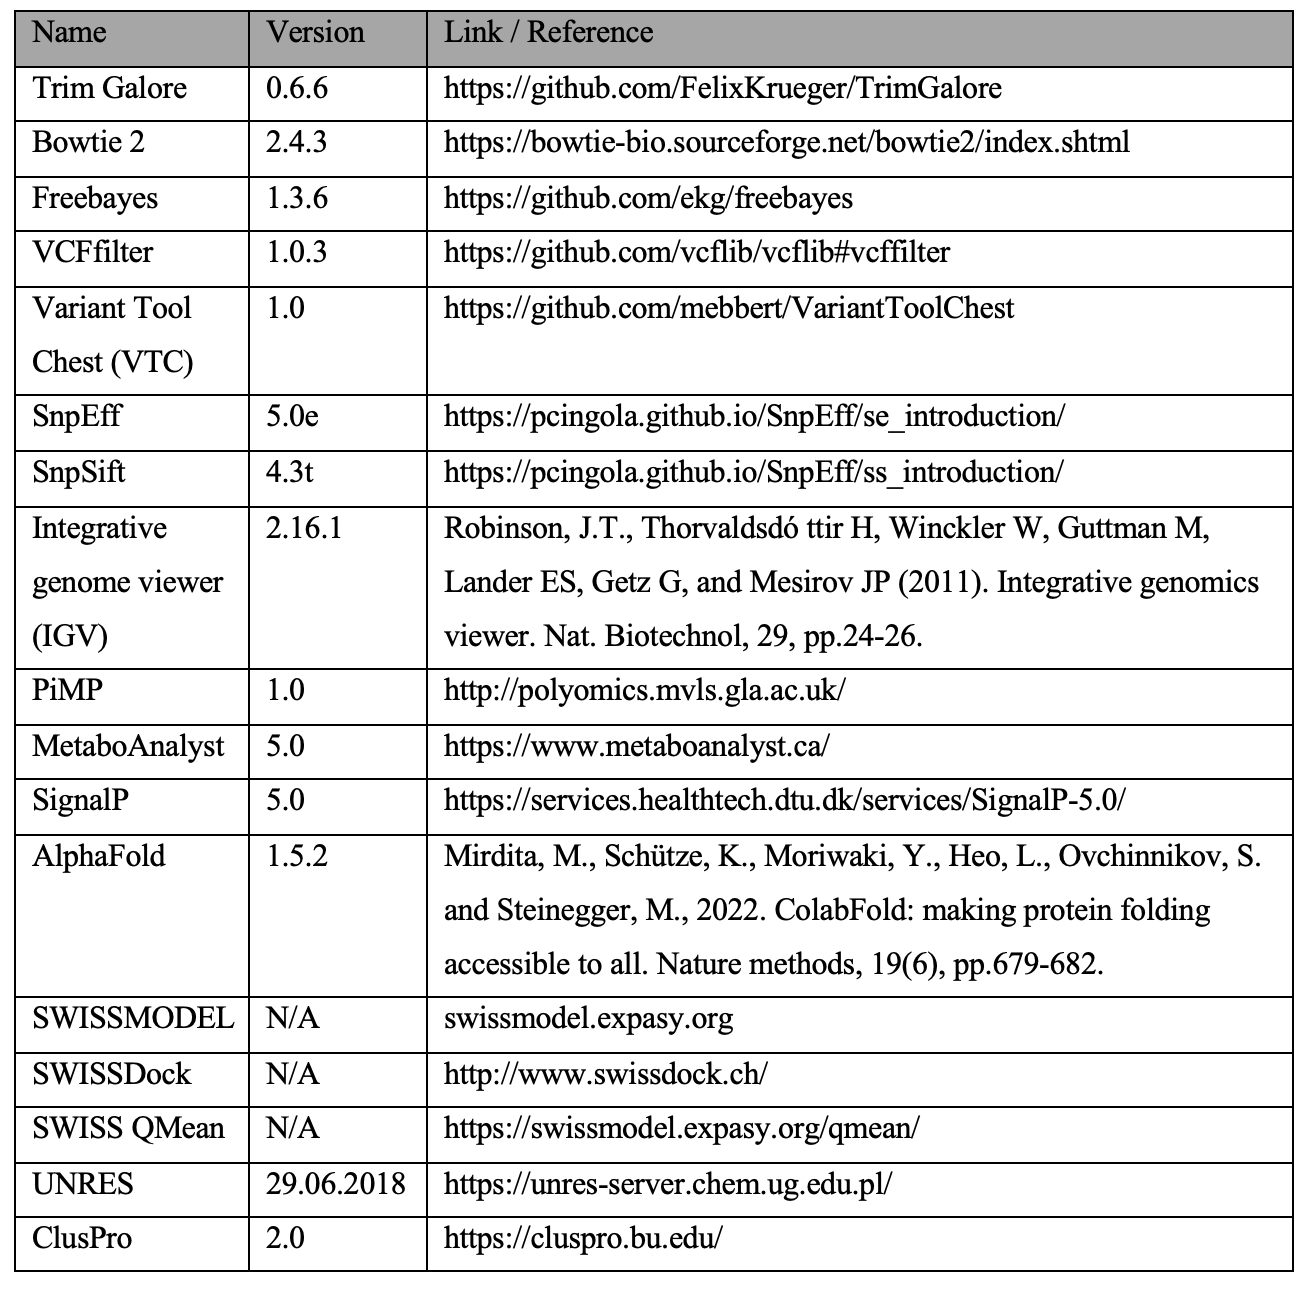
\includegraphics[width=1\linewidth]{Table1} \caption{Summary list of Tools and Programs used in the analysis of the data.}\label{fig:table1}
\end{figure}

\subsection{SNP calling and Effect prediction}

Variants were determined using Freebayes, using default flags, and were
then piped directly to VCFfilter. VCFfilter was used to remove SNPs with
quality scores below 20. Filtered SNPs were put through Variant Tool
Chest to select for SNPs unique to the AmpB resistant line using this
set operator: c{[}data{[}AmpB{]}:data{[}WT{]}{]}. SnpEff then annotates
those SNPs to predict the impact effect of mutations on genes and link
them to the transcript they impact. SnpSift was used to filter for
moderate to high effects, where missense mutations have moderate effects
and stop-gained, frame-shift mutations have high effects. This then
outputs the AmpB resistant compliment SNPs to a VCF file, with this
format: Chromosome, SNP position, ID, Reference allele, Alt allele,
Impact type, Transcript code, Variant in HGVS (DNA) notation, and
Variant in HGVS (protein) notation.

\subsection{SNP UTR region associator}

A custom Python script was written to associate SNPs with putative UTR
regions. The script uses the gffutils library to create a database of
transcript coordinates. It then iterates through a list of SNP
coordinates from the vcf file generated from the SnpEff/Sift tools. The
script then checks if the SNP resides within 200bp upstream of the
transcript start or 500bp downstream of the transcript end. These UTR
lengths were estimated by Dillon et al.~(2015) in \emph{L. major}. It
then writes the SNP position in the chromosome and the transcript code
it affects to a text file.

\subsection{TriTrypDB}

TritrypDB was used to get transcript product descriptions from the
transcript codes that are outputted by SnpSift and our custom Python UTR
code. A list of product descriptions, transcript position was generated
using the search tool : Identify Genes based on List of IDs.

\subsection{Metabolomics}

Metabolomics data was generated using an LC-MS untargeted metabolomics
approach. Four replicate cell extracts per group were taken during their
mid-log phase. Then were processed for separation and mass detection
using HILIC separation column and Orbitrap Exactive mass spectrometer
(Mwenechanya et al., 2017). The metabolomics data was initially
processed using Glasgow Polyomics' PiMP web platform. This enabled us to
differentiate and annotate peaks, according to the Metabolomics Standard
Initiative, and were mapped to KEGG metabolomic maps. This also
calculated log-fold changes, adjusted P-values, and Log odds between our
two groups.

Peak m/z ratios for each replicate were then further processed using the
MetaboAnalyst web platform. This was done to conduct further statistical
analysis of our data. We used their one-factor statistical analysis
module, which replaced missing data with 1/5 of the minimum positive
values, as some statistical tests can't handle missing values. Variables
that are constant between groups are determined using the interquartile
range were filtered to aid compute time and improve statistics; the data
was also log-10 normalised. This data was then used to generate volcano
plots and peak pattern correlation plots were done, correlation
coefficients were calculated using Pearson R test.

\subsection{Proteomics}

Firstly, we downloaded protein sequences for Sterol 14-\(\alpha\)
demethylase (CYP51), ACU00618.1, and Sterol reductase (SR),
XP\_003878080.1. SignalP 5.0 was used to determine the presence of
signal peptides in our protein sequences and their cleavage sites.
Signal peptides were cleaved in CYP51, and none were found in SR.\\

To determine the structures of CYP51 and SR, a few protein modelling
tools were used to determine the yet to be characterised structure of
CYP51 in \emph{L. mexicana} based on the \emph{L. infantum} structure as
a template (PDB code: 3L4D). Models were generated using Alphafold
(Mirdita et al., 2022), Swissmodel (Waterhouse et al., 2018), and Phyre2
(Kelley et al., 2015) on their default settings. Models were quality
checked using SWISS-Model QMEANDisCo method.\\

Substrate docking modelling was carried out with SwissDock, where
Obtusifoliol was used as the substrate in the modelling as it resembles
the true substrate 4,4-dimethylcholesta-8,14,24-trien-3\(\beta\)-ol.
These docking simulations were carried out with wildtype (WT) and mutant
(MT) models of CYP51 to determine the most energetically favoured
position, measured in \(\Delta\)G (kJ/mol).\\

Molecular dynamic modelling was carried out using the UNRES server,
using the predicted structure of CYP51 (WT or MT) and the most
energetically favoured position of the substrate. The modelling was
carried out using the default settings.\\

Protein-protein interaction simulations were carried out with ClusPro.
The structure of Sterol reductase (LmxM.31.2320) was determined using
Alphafold, as there was no related and experimentally determined
structure on the PDB. Both the WT and MT versions of the structures of
CYP51 and SR were used for the interaction simulations on default
settings. The first model from the balanced category were used for
analysis for both WT and MT versions.

\section{Results}

\subsection{Genomics}

Sequencing of the WT and AR lines generated 17.5 million and 15 million
paired reads using Illumina GAIIx sequencing platform. Once processed by
the genomics pipeline outlined in our methods, on average 14\% of the
reads were quality trimmed before alignment using Bowtie 2 (Figure 2 and
3). Due to the inherent plasticity of the Leishmanial genome only an
average of 22\% of the reads were aligned to reference genome. This
plasticity and tendency for the presence of irregular aneuploidy in the
genome would explain the lower alignment, seen in Figure 2 (Negreira et
al., 2022).\\

\begin{figure}
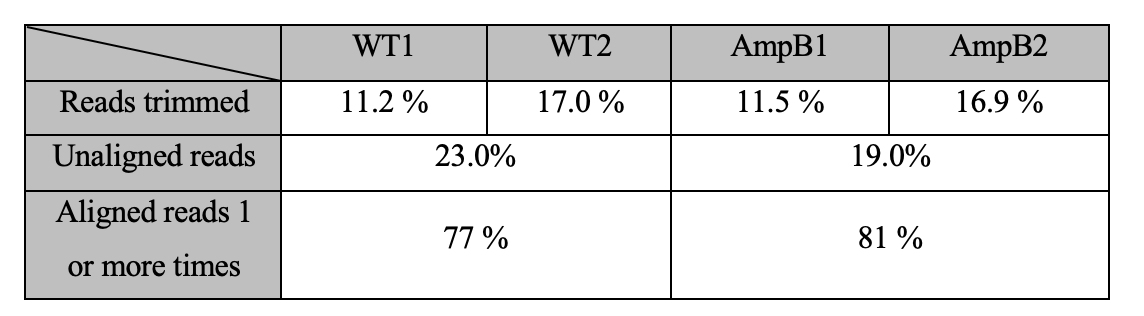
\includegraphics[width=1\linewidth]{Table 2} \caption{Genomics Statistics for TrimGalore and Bowtie2}\label{fig:table2}
\end{figure}

The next step in our pipeline was to visually inspect the aligned BAM
files, using IGV, to verify for any large errors that may have occurred
during alignment. The BAM files of WT and AR were merged, and SNPs were
identified using Freebayes. SNPs were filtered for quality and VTC was
used to select for mutations unique to the AR lines. From this 1132 SNPs
were found to be unique to the AR lines, of which 61\% were either
hetero / homozygous for alternative allele, 22\% were homozygous for the
reference, and 17\% had missing call information.\\

\begin{figure*}[ht]
\center
\includegraphics[width=\textwidth]{"Fastqc trimming.pdf"}
\caption{\label{schema}Figure 1. FastQC of both raw and trimmed paired reads. Phred64 score on the y-axis and base position on the x-axis. Here we can see TrimGalore improved the quality of the 5' end of the paired reads. The average Phred score of both pairs is displayed here.}
\end{figure*}

The snpEff / Sift tools were used to allocate SNPs to the transcripts
they were affecting and those that had moderate to high impact were
selected. Moderate impact SNPs were either missense variants or in frame
deletions; and high impact SNPs were either stop gained or frameshift
variants. In our case, only missense and stop gained mutations were
detected. This gave us shortlist of 134 SNPs, 9 of which were high
impact, that affected 89 transcripts. However, 44 of these transcripts
were described as conserved hypothetical proteins on the TritrypDB
database.\\

We will present here the key SNPs within the shortlist that are relevant
to drug resistance and the ergosterol pathway. These SNPs have all
caused missense mutations in transcripts related to ABC transporters
(LmxM.11.1220/ 1240/ 1290), a nucleoporin (LmxM.28.3030), iron
transporters (LmxM.30.3060 / 3070), and CYP51 (LmxM.11.1100). Two other
transcripts were also affected by missense mutations: Sphingosine kinase
(LmxM.26.0710.1) and 5'-AMP-activated protein kinase catalytic subunit
alpha (LmxM.08\_29.2020.1); that are both involved in the sphingolipid
pathway, an alternate structural lipid.\\

Since UTR regions in Leishmanial genomes have yet to be characterised,
none of the SNPs could be associated to those regions. Using the custom
Python script described in the method, we managed to associate 6\% of
the SNPs to these putative UTR regions. 63 UTR SNPs have potentially
affected 42 genes although only two are of interest, Acyl CoA synthetase
(LmxM.03.0230) and acetyltransferase (LmxM.03.0130). These two proteins
are involved in the fatty acid biosynthesis pathway.

\subsection{Metabolomics}

We conducted an analysis of LC-MS untargeted metabolomics from cell
extracts from our wildtype and AR lines. This generated data on 2811
metabolites from 3144 peaks. However, when comparing the peaks between
WT and AR lines, only 369 peaks are found to have significantly
different log fold changes (Figure 4). One of the peaks that had the
highest log fold change was peak 1051, where low abundance was detected
in the WT sample whereas a great relative abundance was detected in AR.
PiMP has attributed the peak to
4,4-dimethylcholesta-8,14,24-trien-3\(\beta\)-ol, the product of CYP51,
although other sterols such as corbisterol and dehydroconicasterol, were
also attributed.\\

\begin{figure}
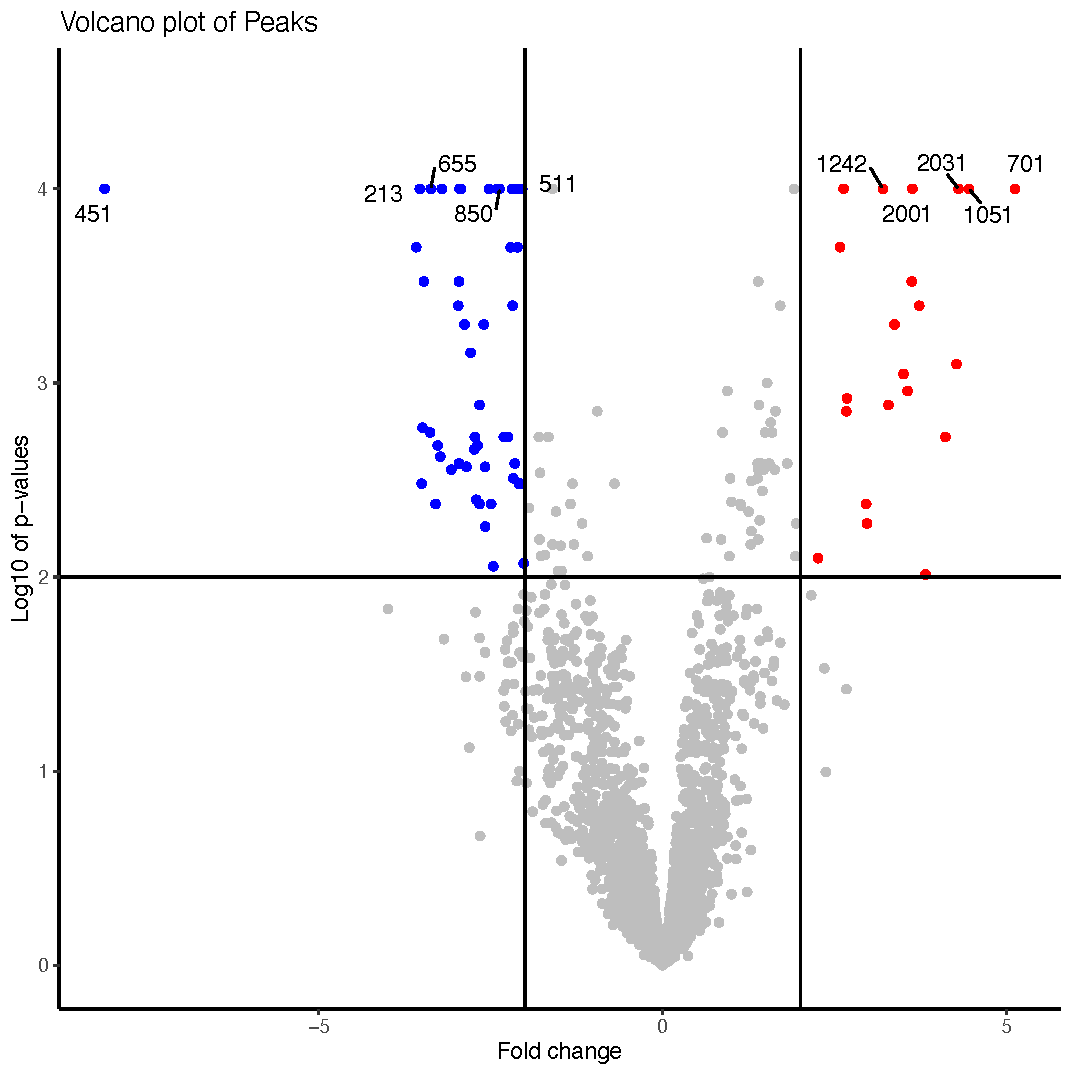
\includegraphics[width=1\linewidth]{volcano} \caption{A volcano plot of LC-MS peak log-fold changes against log-10 transformed P-values. Upregulated peaks are highlighted in red, downregulated peaks are highlighted in blue, and non-significant peaks are left in grey. Significant peaks have a log-fold change > 2 and an adjusted P-value < 0.01. }\label{fig:figure2}
\end{figure}

Correlation analysis of peaks were conducted using the PatternHunter
function on MetaboAnalyst, the correlation distance was calculated using
Pearson r correlation (Figure 5). When running a correlation analysis of
peak 1051, we find that peak 701 is highly correlated. It has an m/z
ratio of 395.4, which could represent a dehydrated form of peak 1051,
since that is the m/z difference of H\textsubscript{2}O (18 m/z). Peak
2031 is another related peak, with a m/z of 387. This peak could
represent cholesterol as it has the same atomic weight; however, many
peaks in our data are near that m/z ratio. Finally, Peak 705 (454 m/z)
was also correlated and was annotated as stigmasterol as well as other
sterols.\\

\begin{figure}
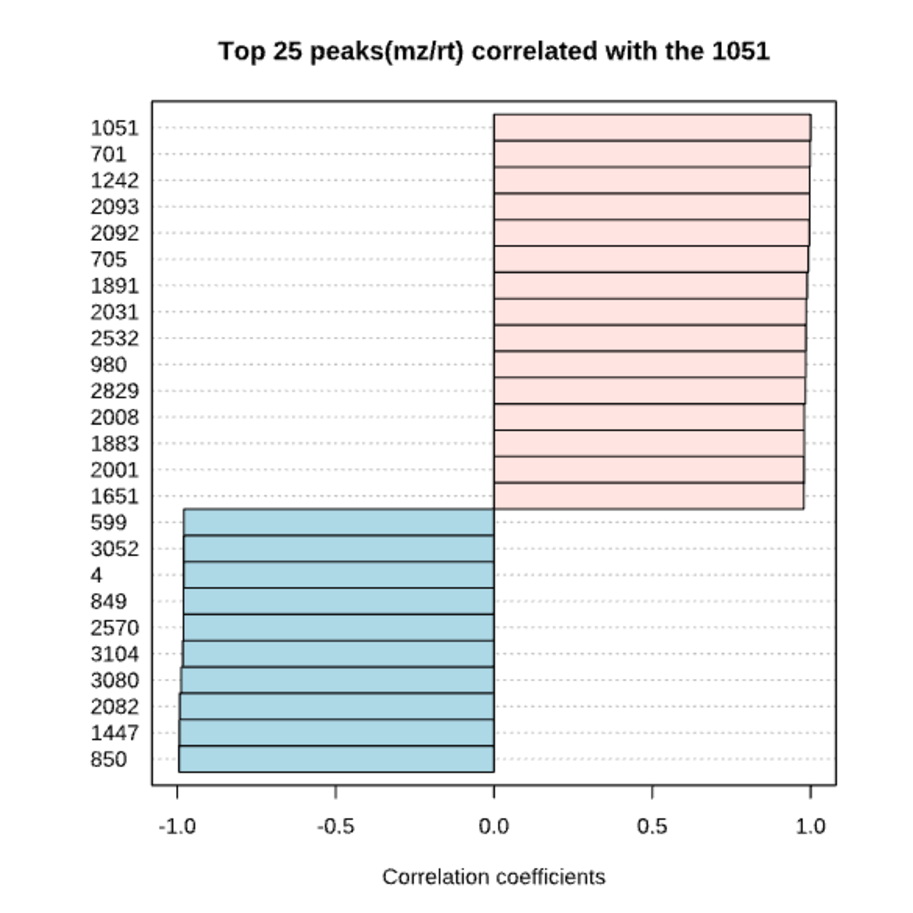
\includegraphics[width=1\linewidth]{1051 correlation table} \caption{Pattern Hunter peak correlation table of 1051. This shows the LC-MS peaks that are closely correlated profiles to 1051 in red, using a Pearson R correlation test. In blue are peaks that have uncorrelated profiles to peak 1051.}\label{fig:figure3}
\end{figure}

The next set of peaks we will present are those that have a lower
relative abundance compared to WT lines. Peaks 451, 502 show a lower
relative abundance, with other related peaks, being annotated as
Ceramides and Glycerophosphocholine. These along with Peaks 516 and
1692, that have a higher relative abundance to WT, all belong to the
sphingolipid biosynthesis pathway (Zhang and Beverley, 2009). Peak 516
was identified as ethanolamine phosphate and 1692 was annotated as
CDP-choline. Peak 1902 was annotated as hexose-phosphates which were
lower in AR lines by 3-fold changes. All the peaks presented here can be
found in Figure 6, with possible metabolite annotations, p.adjusted
values, Log-fold changes, and Log Odds.

\begin{figure}
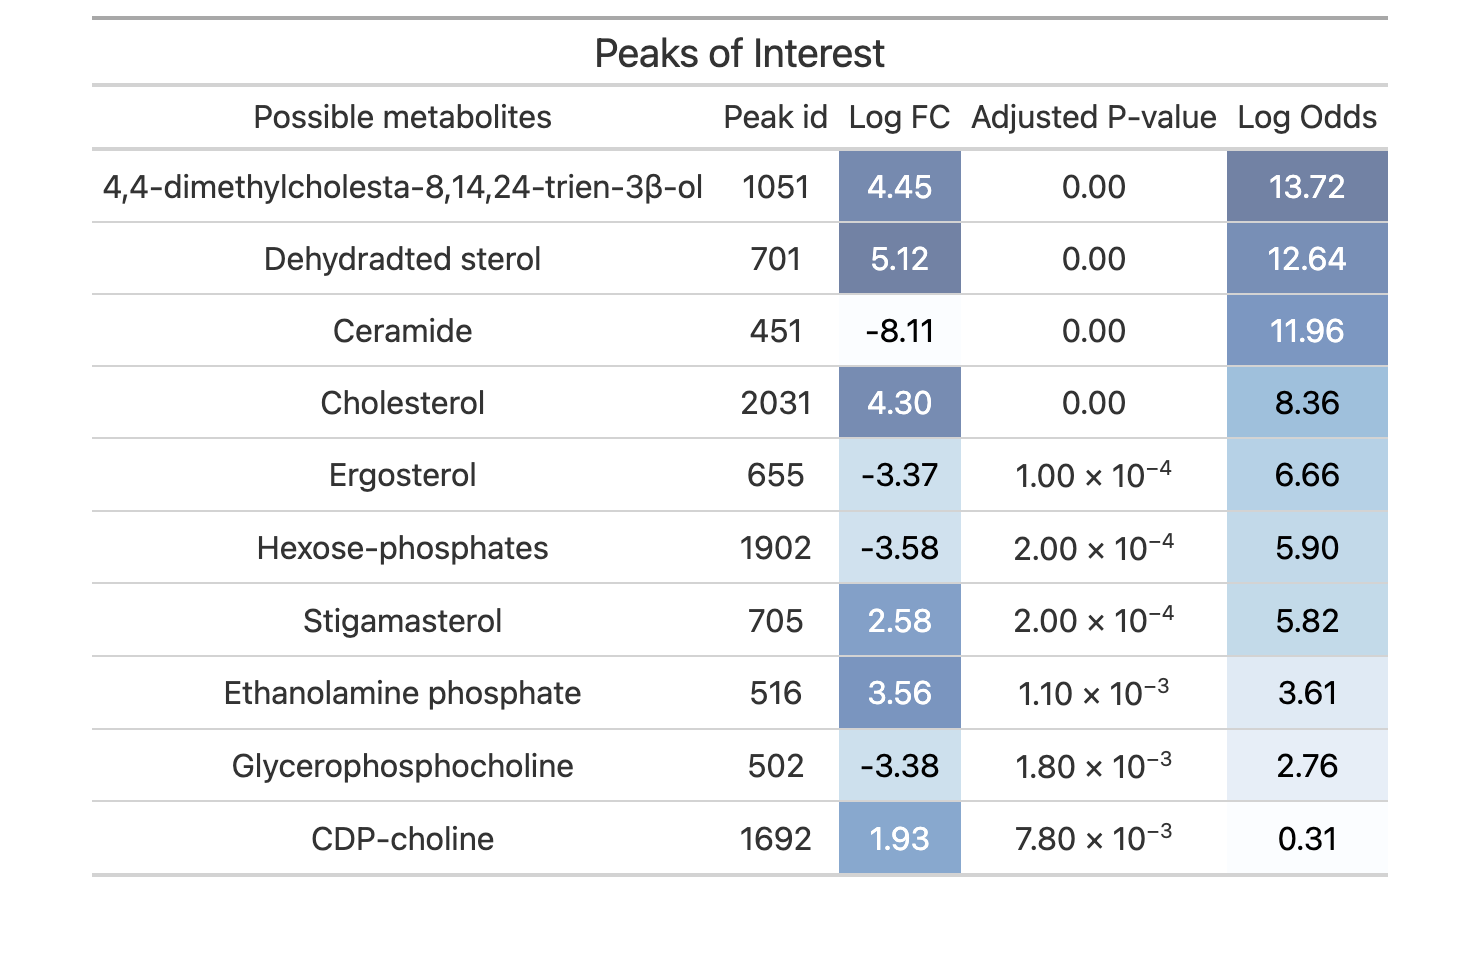
\includegraphics[width=1\linewidth]{peaks of interest} \caption{Summary table of peaks of interest.}\label{fig:figure4}
\end{figure}

\subsection{Structural Proteomics}

Next, we decided to model the point mutation found in CYP51 to determine
its effect on the structure and ligand binding affinity. Since there is
no structure for CYP51 from \emph{L. mexicana} on the PDB, we had to use
model prediction using the structure from \emph{L. infantum} as a
template. \emph{L. infantum} was used as the template because the
Smith-Waterman protein alignment showed a 97 \% identity and 99 \%
similarity. Prior to predicting the models, we checked for signal
peptide cleavage sites in the sequence using SignalP. We decided to trim
the protein sequence at the position 23 cleavage site peak.\\

Here we used AlphaFold, Swissmodel, and Phyre2 to model monomers of both
the WT and MT CYP51 structures. These were compared against each other
to verify for any errors, seen in Figure 7. We can see that the models
align to the template, with the main differences coming from the loop
structures. We chose the AlphaFold model for later analyses although all
models had an QMEANDisCo model quality score of 0.81 ± 0.05.\\

\begin{figure}
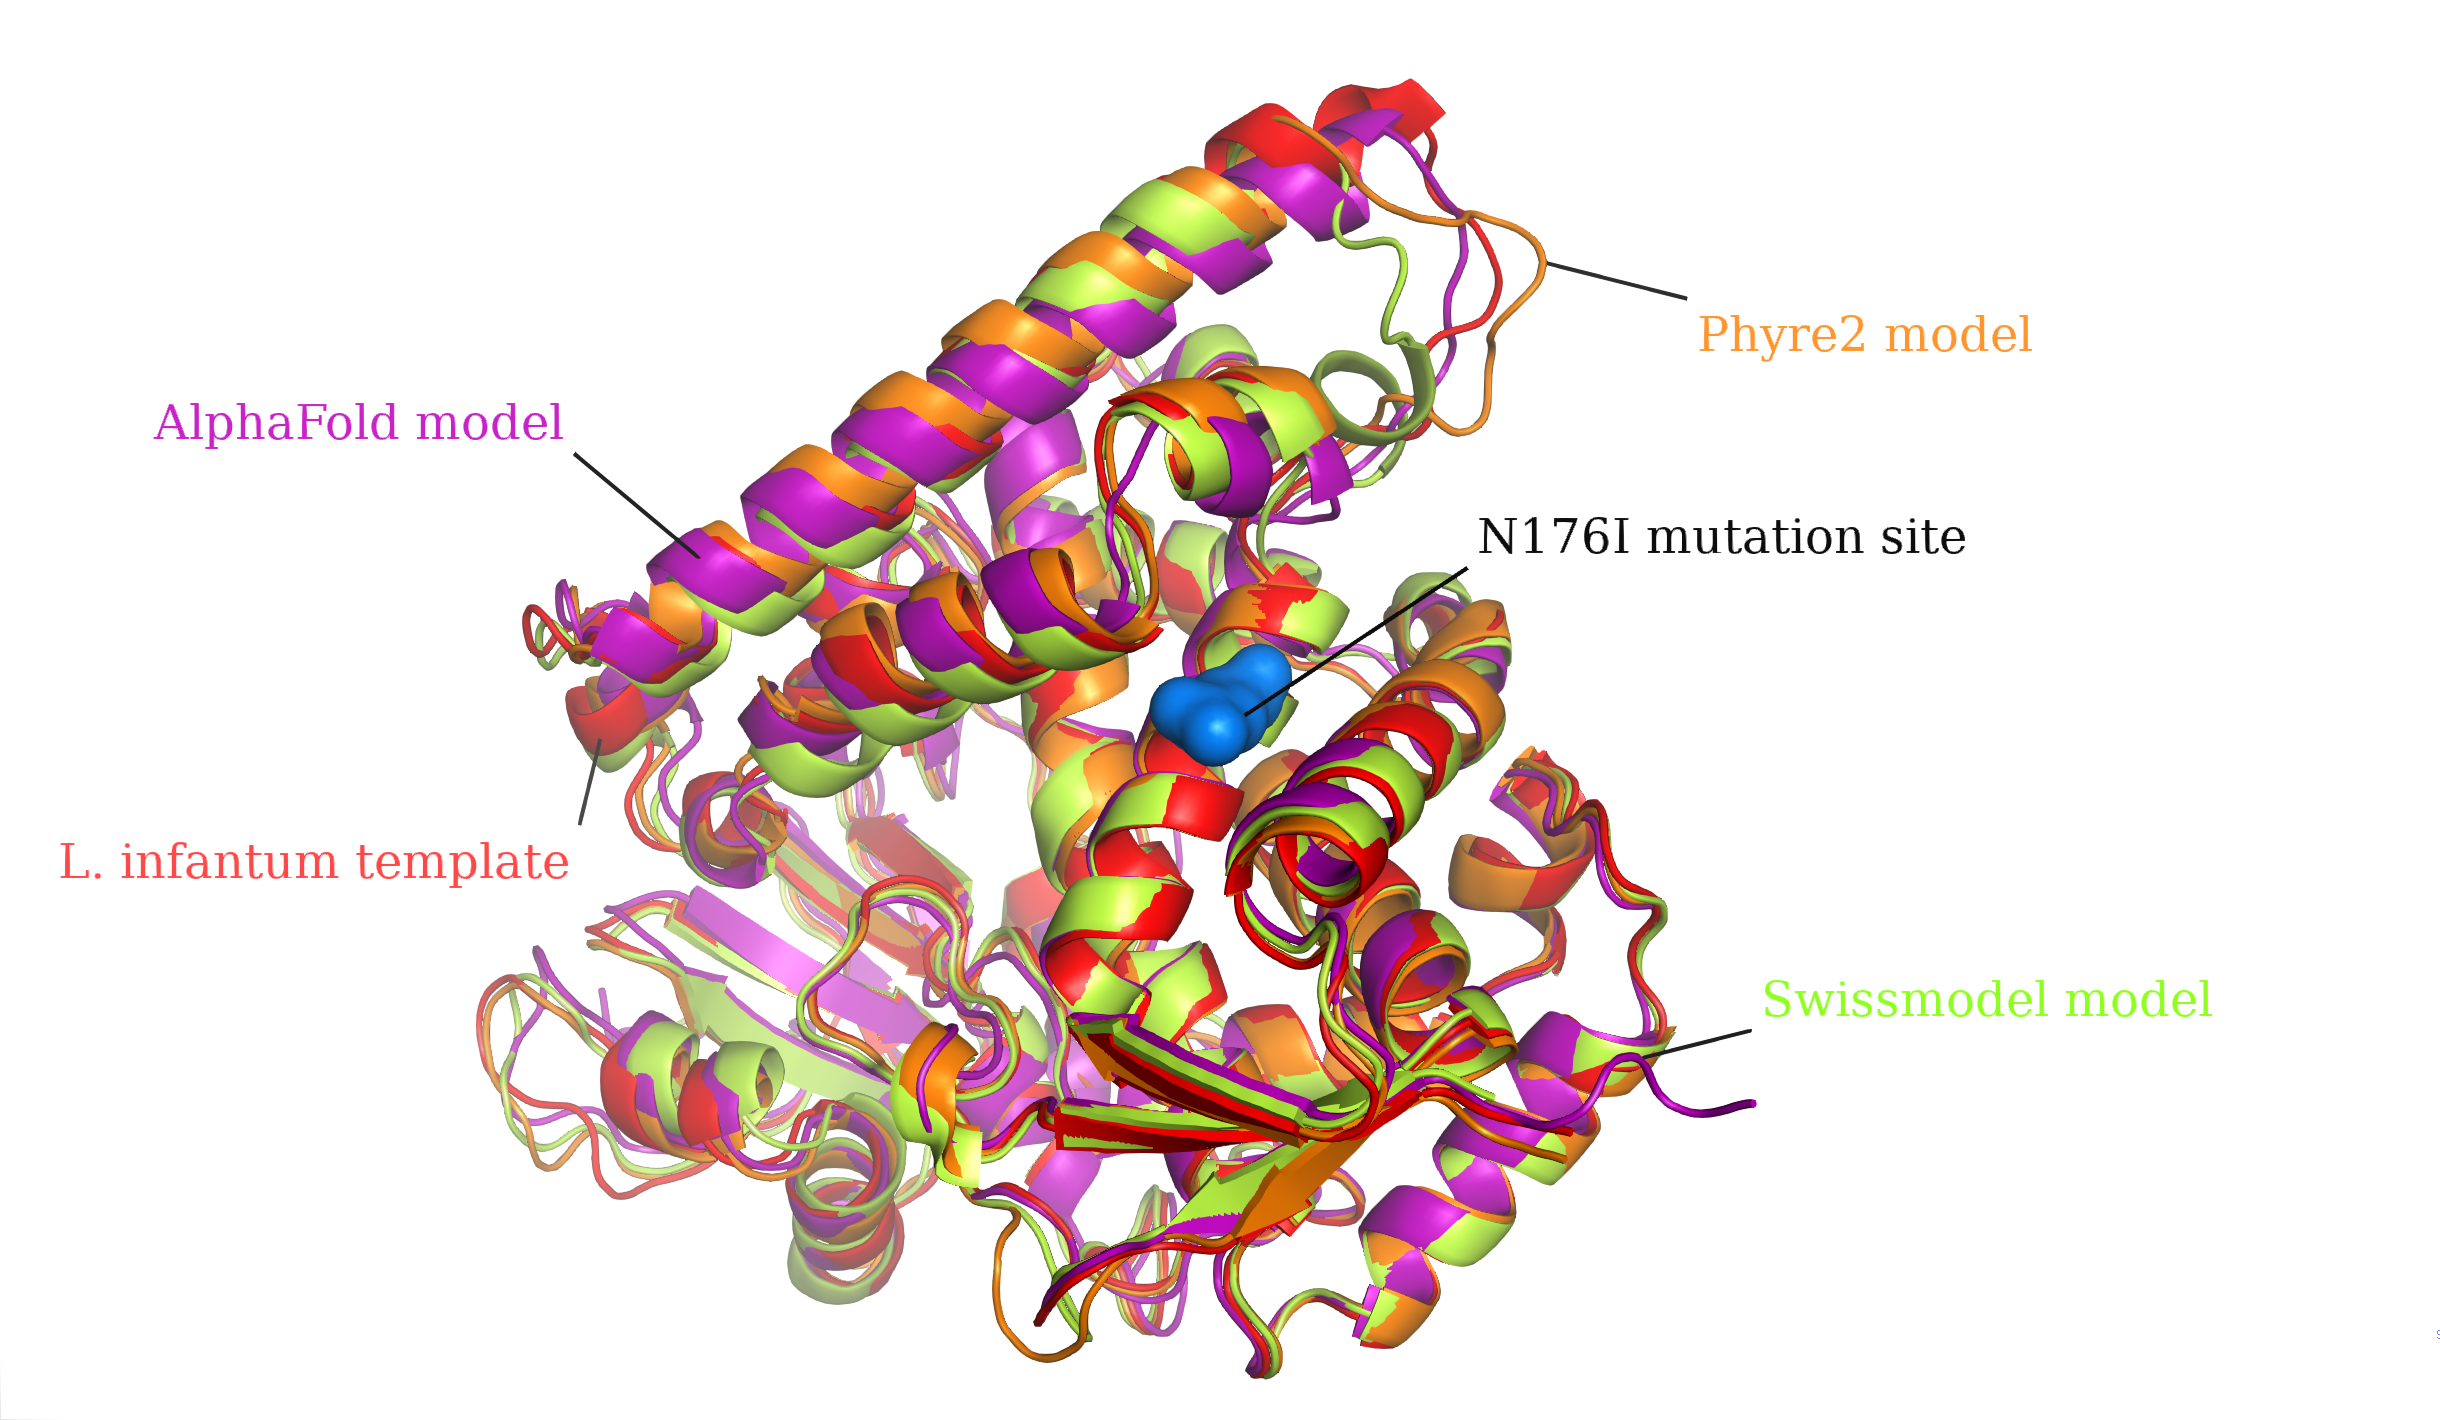
\includegraphics[width=1\linewidth]{model comparison} \caption{CYP51 protein modelling comparison. Here we have the L. infantum template (red), AlphaFold (purple), Phyre2 (orange), and Swissmodel (green) CYP51 models all superimposed. This superimposition and annotations were done in PyMol.}\label{fig:figure5}
\end{figure}

We then ran molecular docking simulations with the enzyme ligand,
14\(\alpha\)-dimethyl-5\(\alpha\)-ergosta-8,24(28)-dien-3-\(\beta\)-ol,
using both the WT and MT AlphaFold models on SWISSDock. We chose the
simulated ligand position that had the lowest \(\Delta\)G (Gibbs free
energy), indicating the difference in thermodynamic states caused by
ligand binding. This represents the binding site that is most
energetically favourable.\\

\begin{figure}
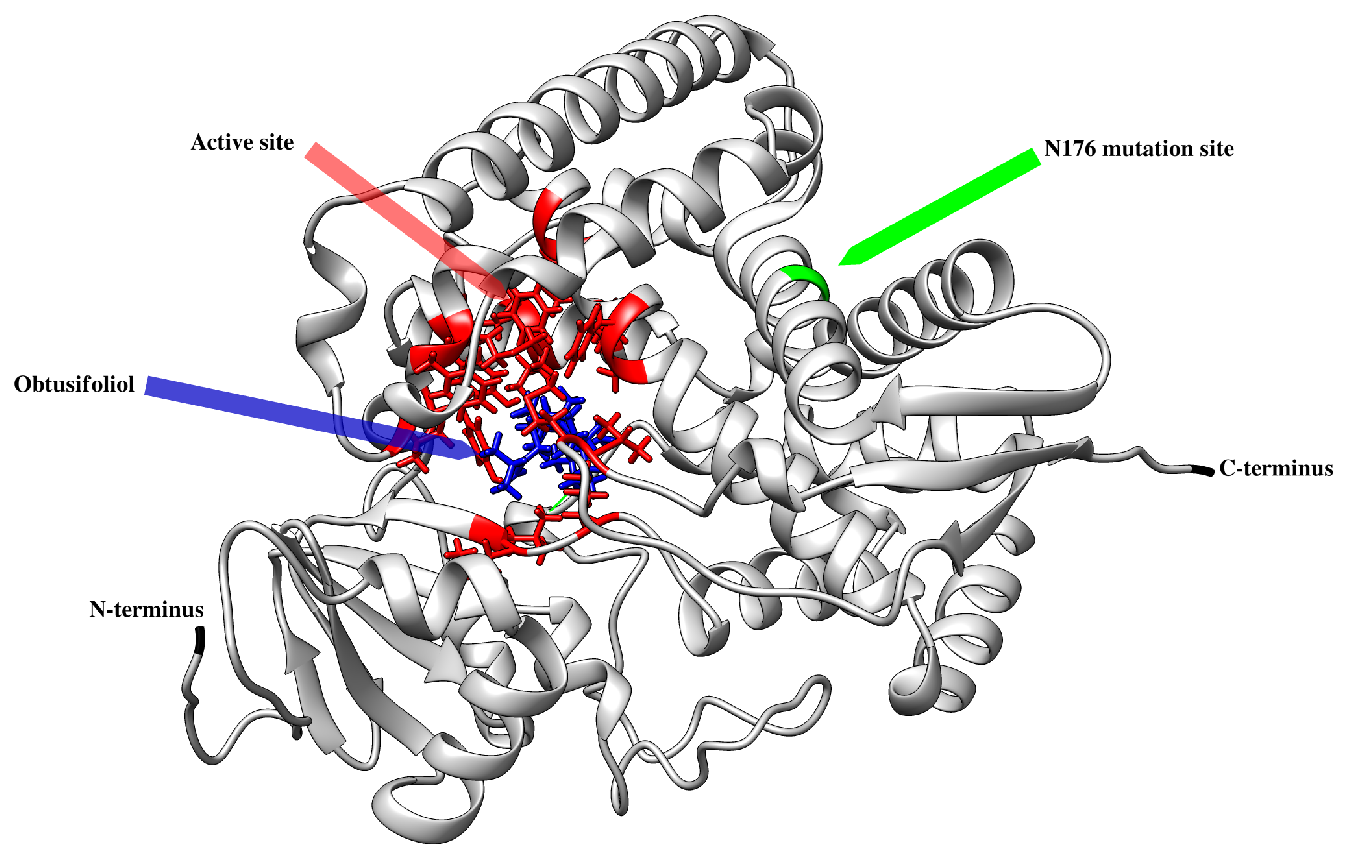
\includegraphics[width=1\linewidth]{CYP51 substrate interaction} \caption{Substrate docking of CYP51 with 14 alpha-dimethyl-5 alpha-ergosta-8,24(28)-dien-3-beta-ol. The active site of the enzyme is highlighted in red, ligand in blue, and the N176I mutation in green. The distance between the closest residue in the active site and N176I was calculated to be ~15 Angstroms. Annotations were done in PyMol.}\label{fig:figure6}
\end{figure}

We then used this docking position in the molecular dynamics' simulation
using the UNRES server, this was done to detect changes in protein
conformation and flexibility. In Figure 9.a), we can see that there is a
difference in the radius of gyration between the WT and MT. Radius of
gyration is a measure of the compactness of a protein, where the smaller
the radius the more compact the protein. As the simulation runs, we see
that the radius of gyration is significantly different and larger in the
MT compared to the WT; showing that the MT is less compact. The
difference in potential energies between two proteins were significantly
different, where the MT has a lower potential energy (Figure 9.b). The
potential energy in the simulation is like \(\Delta\)G and shows the
lowest energy at 300 K; this represents the most likely shape of the
protein at that temperature. (Liwo et al., 2007).\\

\begin{figure*}[ht]
\center
\includegraphics[width=0.7\textwidth]{"bigger dynamics.pdf"}
\caption{\label{schema}Molecular dynamic statistics from UNRES. a) Radius of Gyration ($\mathring{A}$) of both WT and MT CYP51 over Time (picoseconds). b) Potential energy (kcal/mol) of both WT and MT CYP51 over Time (picoseconds). Trendlines were estimated using Local Polynomial Regression Fitting, T-tests were used to determine significance, and variation was determined by standard deviation.  Mutant protein data points coloured in blue, wildtype in red.}
\end{figure*}

The final analysis was the protein -- protein interaction between CYP51
and SR using Cluspro. We wanted to determine any difference in their
interaction and binding affinities caused by the mutation. In Figure
10., we see the top balanced interaction model, where it balances
between hydrophobic and electrostatic interactions, for both WT and MT
CYP51. We can see the interacting surfaces highlighted with their
calculated surface area labelled above. We can also see the distance
between the mutation and the closest amino acid in SR (Valine 188).
There is an approximate 9\% decrease in the interacting surface between
both proteins with the MT CYP51, as well as a greater distance
(4\(\mathring{A}\)) between the proteins towards the N-terminus of
CYP51.

\begin{figure*}[ht]
\center
\includegraphics[width=\textwidth]{"p-p interactions.png"}
\caption{\label{schema}CYP51 and Sterol reductase protein-protein interaction. Here we have the top balanced interaction model from ClusPro using both the WT and MT CYP51 and the Alphafold model of SR. On the left, WT CYP51 interacting with SR with interaction surfaces highlighted along with N176I mutation point (green) and on the right, MT CYP51. The distance between the mutation point and closest residue in SR, Valine 188 is also shown. Interaction surfaces and residue distances were calculated using Pymol.}
\end{figure*}

\section{Discussion}

We will begin our discussion with the main candidate that accounts for
the resistance seen in the AR lines. From our genomics results, we
identified a single missense mutation, asparagine to isoleucine at
position 176 (N176I), in the CYP51 enzyme.\\

In our metabolomics results, we see can that the activity of the enzyme
is not affected by this mutation since we can observe its product, Peak
1051 and 701, however the rest of the ergosterol pathway appears to be
disrupted, as seen in the -3.4 fold change of peak 655. Due to the
limitations of HILIC LC-MS, certain metabolites have co-eluted at the
same time and has made it difficult to separate some peaks. However, we
can be confident that Peaks 1051 and 701 are products of CYP51 due to
their m/z ratios and the fact they have accumulated in AR lines and only
have minimal traces in the WT lines.\\

In protein structure results, we see that the mutation is far from the
active site, \textasciitilde{} 15 \(\mathring{A}\) (Figure 8), and
resides in the proximal N terminus. Our molecular dynamics shows us that
the MT CYP51 has a less compact conformation and has increased
flexibility; this corroborates findings by Vijayakumar and Das, 2018.
This led to us to investigate the protein-protein interaction between
CYP51 and subsequent enzyme, SR. Using the modelling software ClusPro,
it predicted possible surface interactions between the two. Our
modelling showed us that there appears to be some disassociation caused
by the mutation, even though the mutation isn't within these predicted
interaction surfaces in our models (Figure 10). This would imply that
the increased flexibility of the MT CYP51 causes lower binding affinity
to SR. A caveat should be made here, as powerful as these \emph{in
silico} experiments are, CYP51 and SR structures came from protein
modelling algorithms. These interactions are predictions based on
predictions, to be truly confident in our results, we would need to
determine the real structure of both these proteins with
x-crystallography experiments. We could use Co-immunoprecipitation using
antibodies to extract the protein complexes and then use Cryo-Em to
determine their structure; a protocol can be adapted from Cooney et
al.~(2023).\\

The concept of the ergosome that has been characterised by Mo and Bard
(2005) where enzymes involved in ergosterol pathway form a central
enzyme complex. Since both S. cerevisiae and \emph{Leishmania spp.} use
this pathway extensively, it is possible that an ergosome is present in
\emph{Leishmania spp.} This core of enzymes includes CYP51 and SR and
the core is attached to the ER by a scaffolding protein. There is
evidence that this mutation could be causing a disassociation of this
complex by either causing lowered binding affinity with its partners or
perhaps the scaffold protein. However, the ergosome has yet to be fully
characterised in \emph{Leishmania spp.} and it would require an \emph{in
vitro} or \emph{in silico} experiment of multiple protein -- protein
interactions to determine the effect of the N176I mutation.\\

Another potential set of SNPs could be contributing to the resistance,
are the ones affecting the two enzymes in the sphingolipid pathway shown
in the genomics section. Evidence of changes in this pathway can be seen
in Figure 6., where Ceramide / Glycerophosphocholine have decreased in
abundance and Ethanolamine phosphate / CDP-choline have increased. This
suggests that AR lines are using ceramides to potentially produce either
phosphatidylcholines (PC) or phosphatidylethanolamines (PE). The
increased prevalence of both PCs and PEs in drug-resistant lines have
been found before (t'Kindt et al., 2010; Gutierrez Guarnizo et al.,
2021). Both papers have found that these phospholipids contribute to
drug resistance by helping Leishmania spp. to deal with oxidative stress
caused by damage to the mitochondrial membrane. Gutierrez Guarnizo et
al.~(2021), suggest that PC hydrolysis increases the availability of
methyl donor groups that aid against reactive oxygen species. Lastly,
there appears to be increased glucose consumption in AR lines (Figure
6), a similar response was found in a CYP51 KO experiment done by
Mukherjee et al., 2020. They hypothesise that these KOs cause a switch
to the glycolysis pathway for energy consumption and to reduce the
generation of reactive oxygen species.\\

In this report we have shown that a multi-omic approach has the
potential to generate corroborating evidence from different disciplines
that points to the cause of drug resistance in our AR lines. This has
also shown the downsides of using a single drug in targeting a complex
protozoan, perhaps using a synergistic combination of drugs that target
complimentary pathways could vastly decrease the chances of developing
drug resistance. This synergistic combinaation could be determined using
a future multi-omic experiment. The multi-omic approach used here could
help researchers better understand the mechanisms of drug-resistance not
only in Leishmania but other pathogens that are constantly developing
drug-resistances.

\section{References}

Barrett, M.P. and Croft, S.L., 2012. Management of trypanosomiasis and
leishmaniasis. British medical bulletin, 104(1), pp.175-196.\\

Berg, M., García-Hernández, R., Cuypers, B., Vanaerschot, M., Manzano,
J.I., Poveda, J.A., Ferragut, J.A., Castanys, S., Dujardin, J.C. and
Gamarro, F., 2015. Experimental resistance to drug combinations in
Leishmania donovani: metabolic and phenotypic adaptations. Antimicrobial
agents and chemotherapy, 59(4), pp.2242-2255.\\

Cavassin, F.B., Baú-Carneiro, J.L., Vilas-Boas, R.R. and Queiroz-Telles,
F., 2021. Sixty years of amphotericin B: an overview of the main
antifungal agent used to treat invasive fungal infections. Infectious
Diseases and Therapy, 10, pp.115-147.\\

Cerqueira, G.C., Cheeseman, I.H., Schaffner, S.F., Nair, S.,
McDew-White, M., Phyo, A.P., Ashley, E.A., Melnikov, A., Rogov, P.,
Birren, B.W. and Nosten, F., 2017. Longitudinal genomic surveillance of
Plasmodium falciparum malaria parasites reveals complex genomic
architecture of emerging artemisinin resistance. Genome biology, 18,
pp.1-13.\\

Coelho, A.C., Boisvert, S., Mukherjee, A., Leprohon, P., Corbeil, J. and
Ouellette, M., 2012. Multiple mutations in heterogeneous
miltefosine-resistant Leishmania major population as determined by whole
genome sequencing. PLoS neglected tropical diseases, 6(2), p.e1512.\\

Cooney, I., Mack, D.C., Ferrell, A.J., Stewart, M.G., Wang, S.,
Donelick, H.M., Tamayo-Jaramillo, D., Greer, D.L., Zhu, D., Li, W. and
Shen, P.S., 2023. Lysate-to-grid: Rapid Isolation of Native Complexes
from Budding Yeast for Cryo-EM Imaging. Bio-protocol, 13(2).\\

Dillon, L.A., Okrah, K., Hughitt, V.K., Suresh, R., Li, Y., Fernandes,
M.C., Belew, A.T., Corrada Bravo, H., Mosser, D.M. and El-Sayed, N.M.,
2015. Transcriptomic profiling of gene expression and RNA processing
during Leishmania major differentiation. Nucleic acids research, 43(14),
pp.6799-6813.\\

Graf, F.E., Ludin, P., Arquint, C., Schmidt, R.S., Schaub, N., Kunz
Renggli, C., Munday, J.C., Krezdorn, J., Baker, N., Horn, D. and Balmer,
O., 2016. Comparative genomics of drug resistance in Trypanosoma brucei
rhodesiense. Cellular and molecular life sciences, 73, pp.3387-3400.\\

Gutierrez Guarnizo, S.A., Tikhonova, E.B., Zabet-Moghaddam, M., Zhang,
K., Muskus, C., Karamyshev, A.L. and Karamysheva, Z.N., 2021.
Drug-Induced Lipid Remodeling in Leishmania Parasites. Microorganisms,
9(4), p.790.\\

Kelley, L.A., Mezulis, S., Yates, C.M., Wass, M.N. and Sternberg, M.J.,
2015. The Phyre2 web portal for protein modeling, prediction and
analysis. Nature protocols, 10(6), pp.845-858.\\

Kozakov, D., Hall, D.R., Xia, B., Porter, K.A., Padhorny, D., Yueh, C.,
Beglov, D. and Vajda, S., 2017. The ClusPro web server for
protein--protein docking. Nature protocols, 12(2), pp.255-278.\\

Liwo, A., Khalili, M., Czaplewski, C. and Kalinowski, S., 2007. O
ldziej, S., Wachucik, K., Scheraga, HA: Modification and optimization of
the united-residue (UNRES) potential energy function for canonical
simulations. I. Temperature dependence of the effective energy function
and tests of the optimization method with single training proteins.
Journal of Physical Chemistry B, 111(1), pp.260-285.\\

Mirdita, M., Schütze, K., Moriwaki, Y., Heo, L., Ovchinnikov, S. and
Steinegger, M., 2022. ColabFold: making protein folding accessible to
all. Nature methods, 19(6), pp.679-682.\\

Mo, C. and Bard, M., 2005. A systematic study of yeast sterol
biosynthetic protein--protein interactions using the split-ubiquitin
system. Biochimica et Biophysica Acta (BBA)-Molecular and Cell Biology
of Lipids, 1737(2-3), pp.152-160.\\

Mo, C., Valachovic, M. and Bard, M., 2004. The ERG28-encoded protein,
Erg28p, interacts with both the sterol C-4 demethylation enzyme complex
as well as the late biosynthetic protein, the C-24 sterol
methyltransferase (Erg6p). Biochimica et Biophysica Acta (BBA)-Molecular
and Cell Biology of Lipids, 1686(1-2), pp.30-36.\\

Mukherjee, S., Moitra, S., Xu, W., Hernandez, V. and Zhang, K., 2020.
Sterol 14-\(\alpha\)-demethylase is vital for mitochondrial functions
and stress tolerance in Leishmania major. PLoS Pathogens, 16(8),
p.e1008810.\\

Mwenechanya, R., Kovářová, J., Dickens, N.J., Mudaliar, M., Herzyk, P.,
Vincent, I.M., Weidt, S.K., Burgess, K.E., Burchmore, R.J., Pountain,
A.W. and Smith, T.K., 2017. Sterol 14\(\alpha\)-demethylase mutation
leads to amphotericin B resistance in Leishmania mexicana. PLoS
neglected tropical diseases, 11(6), p.e0005649.\\

Negreira, G.H., Monsieurs, P., Imamura, H., Maes, I., Kuk, N., Yagoubat,
A., Van den Broeck, F., Sterkers, Y., Dujardin, J.C. and Domagalska,
M.A., 2022. High throughput single-cell genome sequencing gives insights
into the generation and evolution of mosaic aneuploidy in Leishmania
donovani. Nucleic acids research, 50(1), pp.293-305.\\

Ramos, H., Valdivieso, E., Gamargo, M., Dagger, F. and Cohen, B.E.,
1996. Amphotericin B kills unicellular leishmanias by forming aqueous
pores permeable to small cations and anions. The Journal of membrane
biology, 152, pp.65-75.\\

t'Kindt, R., Scheltema, R.A., Jankevics, A., Brunker, K., Rijal, S.,
Dujardin, J.C., Breitling, R., Watson, D.G., Coombs, G.H. and Decuypere,
S., 2010. Metabolomics to unveil and understand phenotypic diversity
between pathogen populations. PLoS neglected tropical diseases, 4(11),
p.e904.\\

Vijayakumar, S. and Das, P., 2019. Structural, molecular motions, and
free-energy landscape of Leishmania sterol-14\(\alpha\)-demethylase wild
type and drug resistant mutant: A comparative molecular dynamics study.
Journal of Biomolecular Structure and Dynamics, 37(6), pp.1477-1493.\\

Vincent, I.M. and Barrett, M.P., 2015. Metabolomic-based strategies for
anti-parasite drug discovery. Journal of biomolecular screening, 20(1),
pp.44-55.\\

Waterhouse, A., Bertoni, M., Bienert, S., Studer, G., Tauriello, G.,
Gumienny, R., Heer, F.T., de Beer, T.A.P., Rempfer, C., Bordoli, L. and
Lepore, R., 2018. SWISS-MODEL: homology modelling of protein structures
and complexes. Nucleic acids research, 46(W1), pp.W296-W303.


% Bibliography
\bibliographystyle{natbib}
\bibliography{bibliography.bib}

\end{document}
